% For more detailed article preparation guidelines, please see: http://wellcomeopenresearch.org/for-authors/article-guidelines and http://wellcomeopenresearch.org/for-authors/data-guidelines

\documentclass[10pt,a4paper,twocolumn]{article}
\usepackage{WellcomeOR_styles}

%% Packages added manually
\usepackage{float}
\usepackage{hyperref}
\usepackage{booktabs}
\usepackage{longtable}


%% Default: numerical citations
\usepackage[numbers]{natbib}

%% Uncomment this lines for superscript citations instead
% \usepackage[super]{natbib}

%% Uncomment these lines for author-year citations instead
% \usepackage[round]{natbib}
% \let\cite\citep

\begin{document}

\title{Wellcome Open Research Article Template}
\titlenote{The title should be detailed enough for someone to know whether the article would be of interest to them, but also concise. Please ensure the broadness and claims within the title are appropriate to the content of the article itself.}


\author[1, 2, 3]{Anonymous Alpaca}
\author[2]{Benevolent Brachiosaurus}
\affil[1]{Department of Infectious Disease Epidemiology, London School of Hygiene \& Tropical Medicine, London, United Kingdom}
\affil[2]{Centre for the Mathematical Modelling of Infectious Diseases, London, United Kingdom}
\affil[3]{NIHR Health Protection Research Unit in Modelling \& Health Economics}
\affil[2]{Address of author2}


\maketitle
\thispagestyle{fancy}

% Please list all authors that played a significant role in the research involved in the article. Please provide full affiliation information (including full institutional address, ZIP code and e-mail address) for all authors, and identify who is/are the corresponding author(s).



\begin{abstract}

Abstracts should be up to 300 words and provide a succinct summary of the article. Although the abstract should explain why the article might be interesting, care should be taken not to inappropriately over-emphasise the importance of the work described in the article. Citations should not be used in the abstract, and the use of abbreviations should be minimized. If you are writing a Research or Systematic Review article, please structure your abstract into Background, Methods, Results, and Conclusions.

\textbf{Background}

\textbf{Methods}

\textbf{Results}

\textbf{Conclusions}



\end{abstract}

\section*{Keywords}

Human judgement forecasting, COVID-19, infectious disease, 

% Please list up to eight keywords to help readers interested in your article find it more easily.


\clearpage

\section*{Introduction}

Infectious disease modelling and forecasting has attracted wide-spread attention during the COVID-19 pandemic and helped inform decision making in public health organisations and governments \cite{cramerEvaluationIndividualEnsemble2021, venkatramananUtilityHumanJudgment2022}. 
% Beginining in March 2020, forecasts for different COVID-19 targets have been systematically collated by Forecast Hubs in the US \citep{cramerEvaluationIndividualEnsemble2021}, Germany and Poland \citep{bracherShorttermForecastingCOVID192021, bracherNationalSubnationalShortterm2021}, and Europe \citep{sherrattPredictivePerformanceMultimodel2022a}. 
Most forecasts were based on computational models of COVID-19, but some authors also explored human judgement forecasting as an alternative \cite{recchiaHowWellDid2021, mcandrewExpertJudgmentModel2022, bosseComparingHumanModelbased2022, mcandrewChimericForecastingCombining2022}. 

Past research found that in the context of infectious disease forecasting, human judgement forecasts could achieve predictive performance broadly comparable to forecasts generated based on mathematical modelling, in particular when forecasting incident cases. \citet{farrowHumanJudgmentApproach2017} found that an aggregate of human predictions outperformed computational models when predicting the 2014/15 and 2015/16 flu season in the US. However, a comparable approach performed slightly worse than computtional models at predicting the 2014/15 outbreak of chikungunya in the Americas. 
\citet{bosseComparingHumanModelbased2022} found an ensemble of human forecasters to outperform an ensemble of computational models when predicting cases of COVID-19 in Germany, but performing worse when predicting incident deaths. Similarly, \citet{mcandrewChimericForecastingCombining2022} reported an ensemble of human forecasters to perform comparably to an ensemble of computational models when predicting incident cases, and worse when predicting incident deaths. \citet{farrowHumanJudgmentApproach2017} and in particular \citet{bosseComparingHumanModelbased2022} struggled to recruit a large number of participants (numbers of active forecasters ranged from 22 to 61 in \citet{mcandrewChimericForecastingCombining2022}, 7 to 24 in \citet{farrowHumanJudgmentApproach2017}, and 4 to 10 in \citet{bosseComparingHumanModelbased2022}). 

In some situations, human judgement forecasting has clear advantages relative to computational models. Humans can very quickly provide forecasts, even in situations where data is sparse and lots of parameters are unknown. In addition, humans are able to answer a broad set of question (such as for example the likelihood that a given actor will take some specified action) or can take factors into account that are hard to encode in a computational model. On the other hand, human judgement forecasting is difficult to scale due to the time and effort required, and humans may be at a disadvantage at tasks that require complex computations. 


% Beginining in March 2020, forecasts for different COVID-19 targets have been systematically collated by Forecast Hubs in the US \citep{cramerEvaluationIndividualEnsemble2021}, Germany and Poland \citep{bracherShorttermForecastingCOVID192021, bracherNationalSubnationalShortterm2021}, and Europe \citep{sherrattPredictivePerformanceMultimodel2022a}. 

Methods that aim to combine human judgement and mathematical modelling are therefore appealing. One straightforward way is to combine separate human judgement and computational model forecasts with the goal of improving predictive performance \citep{mcandrewChimericForecastingCombining2022}. \cite{farrowHumanJudgmentApproach2017, bosseComparingHumanModelbased2022} and others suggested additional possibilities in the context of infectious diseases that may also help reduce the amount of human effort required. One approach is to use human forecasts, for example of relevant disease paremeters, as an input to computational modelling. Another approach is to use mathematical modelling as an input to human judgement, for example by giving experts the option to make post-hoc adjustements to model outputs. \citet{bosseComparingHumanModelbased2022} proposed to ask human forecasters to predict the effective reproduction number $R_t$ (the average number of people an infected person would infect in turn) and to feed this forecast into a mathematical model in order to obtain forecasts for case and death numbers. 

This paper represents a follow-up study to \citet{bosseComparingHumanModelbased2022} in the United Kingdom with forecasts made over the course of thirteen weeks between May and August 2021. Forecasts were elicited from experts and laypeople as part of a public forecasting tournament, the "UK Crowd Forecasting Challenge" using a web application. All forecasts were submitted to the European COVID-19 Forecast Hub, one of several Forecast Hubs that have been systematically collating forecasts of different COVID-19 forecast targets in the US \citep{cramerEvaluationIndividualEnsemble2021}, German and Poland \citep{bracherShorttermForecastingCOVID192021, bracherNationalSubnationalShortterm2021}, and Europe \citep{sherrattPredictivePerformanceMultimodel2022a}. This study aims to investigate whether the original findings in \citet{bosseComparingHumanModelbased2022} with respect to forecaster performance replicate in a different country and with an increased number of participants. In addition, it explores the approach proposed in \citet{bosseComparingHumanModelbased2022} to ask participants for a forecast of the effective reproduction number $R_t$ which is then translated into a forecast of cases and deaths using a mathematical model. 

% Define the terms model, forecaster, crowd forecast, ensemble. 

\section*{Methods}

\subsection*{Ethics statement}
This study has been approved by the London School of Hygiene \& Tropical Medicine Research Ethics Committee (reference number 22290). Consent from participants was obtained in written form.

\subsection*{Interaction with the European Forecast Hub}

The European COVID-19 Forecast Hub \cite{sherrattPredictivePerformanceMultimodel2022a} elicits predictions for various COVID-19 related forecast targets from different research groups every week. Forecasts had to be submitted every Monday 23.59pm GMT. Forecasts are made for incident weekly reported numbers of cases of and deaths from COVID-19 on a national level for various European countries over a one to four week forecast horizon. While forecasts were submitted on Mondays, weeks were defined as epiweeks. ending on a Saturday and starting on Sunday. Forecast horizons were therefore in fact 5, 12, 19 and 26 days. Submissions to the European Forecast Hub follow a quantile-based format with 23 quantiles of each output measure at levels 0.01, 0.025, 0.05, 0.10, 0.15,…, 0.95, 0.975, 0.99.
Every week, forecast submitted to the hub were automatically checked for conformity with the required forecasta and all eligible forecasts combined into different ensembles. Until the 12th of July 2021 the default Hub ensemble shown on all official Forecast Hub visualisiations (https://covid19forecasthub.eu/) was a mean-ensemble (i.e., the $\alpha$-quantile of the ensemble is given by the mean of all submitted $\alpha$-quantiles). From the 29th of July on, the default Forecast Hub ensemble became a median-ensemble. The number of models included in the Forecast Hub ensemble is shown in Figure \ref{fig:num-forecasters}. 

Ground-truth data on daily reported test positive cases and deaths linked to COVID-19 were provided by European Forecast Hub and sourced from the Johns Hopkins University. Data were subject to reporting artifacts and revisions. The Forecast Hubs marks data as anomalous if in subsequent updates data is changed by more than 5 percent. THIS IS THE CASE FOR ALL DEATH FORECASTS... CAN WE CHECK THIS? 
See Figure MAKE FIGURE WITH DATA AND UPDATES. 

\subsection*{Human judgement forecasts}

Forecasts of incident cases and deaths linked to COVID-19 in the UK were elicited from individual participants every week through the web application (https://cmmid-lshtm.shinyapps.io/crowd-forecast/) described in \cite{bosseComparingHumanModelbased2022}. The application is based on \textsf{R} \cite{R} \texttt{shiny} \cite{shiny} and is available as an \textsf{R} package called \texttt{crowdforecastr} \citep{crowdforecastr}. 

The web application offered participants two different ways of making a forecast called 'direct' (or 'classical') and 'Rt' forecast. To make a 'direct' forecast (as described in more detail \cite{bosseComparingHumanModelbased2022}), participants selected a predictive distribution (by default a log-normal distribution) and adjusted the median and width of the distribution to change the central estimate and uncertainty. In addition to information about past observations, participants could see various metrics and data sourced from Our World in Data \citep{owidcoronavirus}. Figure \ref{fig:screenshot-classical} shows a screenshot of the forecast interface for direct forecasts. 

SAM TO THE RESCUE

In addition, we implemented a second forecasting method ('Rt forecasts'), where we asked participants to make a forecast of the effective reproduction number $R_t$. This forecast was then translated into forecasts of cases using the renewal equation \citep{fraserEstimatingIndividualHousehold2007} as implemented in the \textsf{R} package \texttt{EpiNow2} \citep{epinow2}, APPENDIX INFO?. In order to obtain forecasts for deaths, we convolved predicted infections as implied by the $R_t$ forecast over data-based delay distributions \cite{epinow2, sherrattExploringSurveillanceData2021, abbottEstimatingTimevaryingReproduction2020a} to model the time between infection and report date. As $R_t$-estimates up to two weeks prior to the forecast data were deemed uncertain, we also asked participants to submit an estimate of $R_t$ for the two weeks prior to the current forecast date. Participants were therefore asked to estimate / predict four $R_t$ values, four of them in the future. Upon pressing a button participants could see a preview of the evolution of cases implied by their current $R_t$ forecast. However, due to the high computational complexity and necessary waiting times, participants could not preview the death forecast implied by their current input for $R_t$. Figure \ref{fig:screenshot-rt} shows a screenshot of the forecast interface for $R_t$ forecasts. 

Every week, we submitted an ensemble of individual forecasts ("crowd forecast") to the European Forecast Hub. In contrast to the ensemble of human forecasts described in \citet{bosseComparingHumanModelbased2022}, we used the quantile-wise median, rather than the quantile-wise mean to combine predictions. %, following suggestions made in CITATION. 
We submitted three different ensembles: The first one, "epiforecasts-EpiExpert\_direct" (here called "Crowd direct") was a quantile-wise median ensemble of all the direct forecasts. "epiforecasts-EpiExpert\_Rt" (here called "Crowd Rt" was a median ensemble of all forecasts made through the $R_t$ interface. "epiforecasts-EpiExpert" (here called "Crowd combined") was a median ensemble of all forecasts, after combining direct and $R_t$ forecast from the same individual by taking a quantile-wise mean. Before creating the ensemble, we deleted forecasts that were clearly the result of a user or software error (such as forecasts that were zero everywhere).

\subsection*{EpiNow2?}

SAM TO THE RESCUE, RELEVANT PART OF OLD PAPER PASTED HERE AND COMMENTED OUT. DO WE NEED AN EXTRA SECTION, OR SHOULD THIS BE INCLDUED ABOVE? 

% From old paper: 
% The first of these models, here called “renewal model”, used the renewal equation [41] to predict reported cases and deaths (see details in S1 Text). It estimated the effective reproduction number Rt (the average number of people each person infected at time t is expected to infect in turn) and modelled future infections as a weighted sum of past infection multiplied by Rt. Rt was assumed to stay constant beyond the forecast date, roughly corresponding to continuing the latest exponential trend in infections. On the 9th of November we altered the date when Rt was assumed to be constant from two weeks prior to the date of the forecast to the forecast date, which we found to yield a more stable Rt estimate. Reported case and death notifications were obtained by convolving predicted infections over data-based delay distributions [40, 42–44] to model the time between infection and report date. The renewal model was used to predict cases as well as deaths with forecasts being generated for each target separately. Death forecasts from the renewal model were therefore not informed by past cases. One submission of the renewal model on December 28th 2020 was delayed and therefore not included in the official Forecast hub ensemble.
% 
% Line list data used to inform the prior for the delay from symptom onset to test positive case report or death in the model-based forecasts was sourced from [45] with data available up to the 1st of August. All model fitting was done using Markov-chain Monte Carlo (MCMC) in stan [46] with each location and forecast target being fitted separately.

\subsection*{The UK Crowd Forecasting Challenge}

In order to boost participation compared to our last crowd forecasting study in Germany and Poland \citep{bosseComparingHumanModelbased2022}, we announced an official tournament, the "UK Crowd Forecasting Challenge". Participants were asked to submit weekly predictions for reported cases and deaths linked to COVID-19 in the United Kingdom one to four weeks into the future. Everynone who had submitted a forecast for targets in the UK during the tournament period from the 24th of May 2021 to the 16th of August 2021 was deemed a participant and eligible for a prize. The first prize was 100 GBP, second prize 50 GBP and third prize 25 GBP. For the purpose of the tournament ranking, participants who did not submit a forecast in a given week where assigned the median score of all other participants who submitted a forecast that week. The UK crowd forecasting challenge was announced over Twitter and our networks. 
% (e.g. https://www.voice-global.org/public/opportunities/archived/uk-covid-19-crowd-forecasting-challenge/)
In addition, we created a project website, \url{https://crowdforecastr.org}, made weekly posts on Twitter and sent participants who had registered on the online application weekly emails with a reminder and a summary of their past performance. A public leaderboard was available on our website \url{https://epiforecasts.io}. Participants could choose to make a direct forecast as well as an $R_t$ forecast and were eligible for prizes twice. Weekly forecasts had to be submitted between Sunday 12pm and Monday 8pm UK time. 


\subsection*{Analysis}

Our analysis of the data largely follows the one outlined in \citet{bosseComparingHumanModelbased2022}. If not otherwise stated, we present results for two-week-ahead forecasts, following the practice adopted by the COVID-19 Forecast Hubs that found poor predictive performance beyond this horizon [15]. 

We scored forecasts using the weighted interval score (WIS, formulas given in the SI in Section \ref{sec:wis}) \cite{bracherEvaluatingEpidemicForecasts2021} and used the empirical coverage of all central 50\% and 90\% prediction intervals to measure probabilistic callibration. The WIS is proper scoring rule (with smaller values implying better performance). A forecaster, in expectation, optimises her score by providing a predictive distribution $F$ that is equal to the data-generating distribution $G$ and is therefore incentivised to report her true belief. The WIS can be seen as a generalisation of the absolute error to predictive distribution in a quantile-based format and represents an approximation of the continuous ranked probability score (CRPS). The WIS can be decomposed into three separate penalty components: forecast spread (i.e. uncertainty of forecasts), over-prediction and under-prediction. FORMULAS IN APPENDIX. Empirical coverage means the percentage of observations falling inside any given prediction interval (e.g. the cumulative percentage of observed values that fall inside all 50\% prediction intervals). It represents a measure of probabilistic calibration \citep{gneitingProbabilisticForecastsCalibration2007}. Forecasts were evaluated using the \texttt{scoringutils} \citep{bosseEvaluatingForecastsScoringutils2022} package in \textsf{R}.

\citet{bosseTransformationForecastsEvaluating2023} recently suggested to transform forecasts and observations using the natural logarithm prior prior to applying the WIS in order to better reflect the exponential nature of the underlying disease process. We therefore also compute WIS values after transforming all forecasts and observations using the function $f\colon x \to \log (x + 1)$. In the following, we refer to WIS scores obtained without a transformation as "scores on the natural scale", and WIS values obtained after log-transforming forecasts and observations as "scores on the log scale". 

\section*{Results}

\subsection*{Crowd forecast participation}

A total number of 90 participants submitted forecasts (more precisely, forecasts were submitted from 90 different accounts, some of them anonymous). The median number of unique participants in any given week was 17, the minimum was 6 and the maximum was 51. With respect to the number of submissions from an individual participant, we observed similar patterns as \cite{bosseComparingHumanModelbased2022}: An individual forecaster participated on average in 2.6 weeks out of 13. The median number of submissions was one, meaning that most forecasters dropped out after their first submission. Only five participants submitted a forecast in ten or more weeks and only two submitted a forecast in all thirteen weeks, one of whom is an author on this study. The number of direct forecasts was higher than the number of $R_t$ forecasts in all weeks (see Figure \ref{fig:num-forecasters}). 

% X of those self-identified as ‘expert’ in either forecasting or epidemiology. 

\begin{figure}[H]
\centering
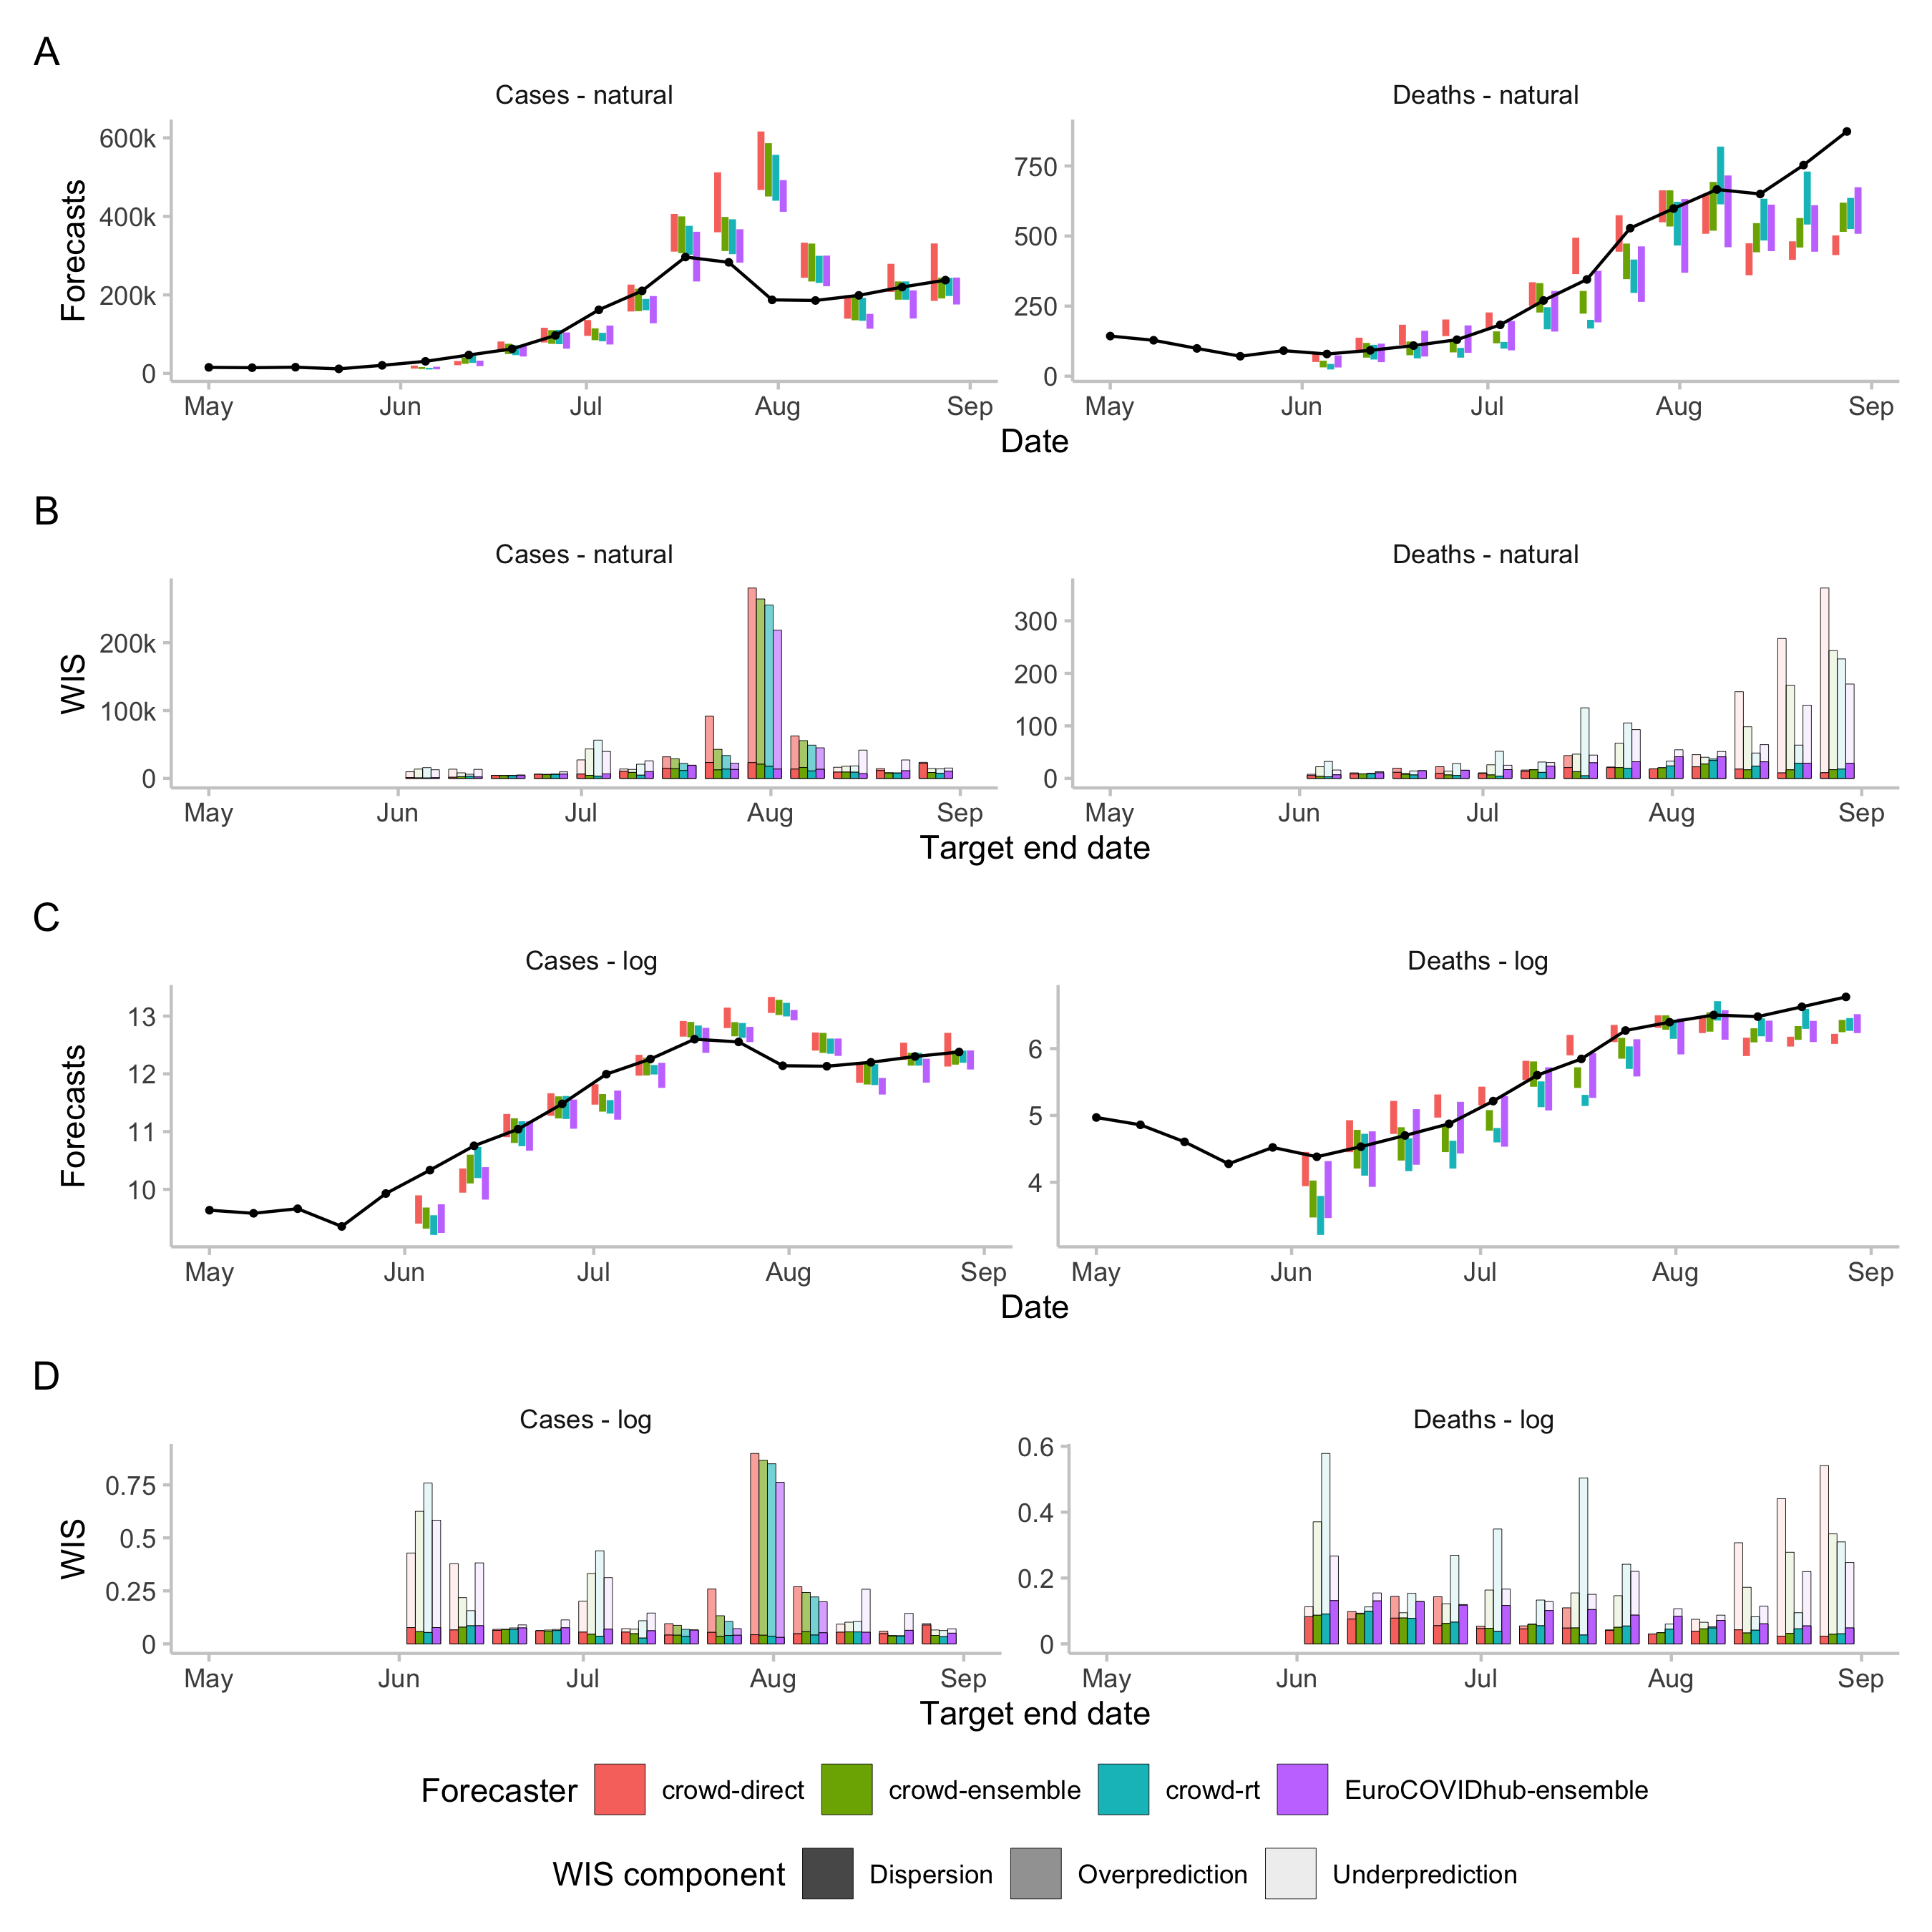
\includegraphics[width=0.99\textwidth]{../output/figures/scores-and-forecasts.png}
\caption{\bf{Test}}
\label{fig:forecasts-scores}
\end{figure}


\begin{figure}[H]
\centering
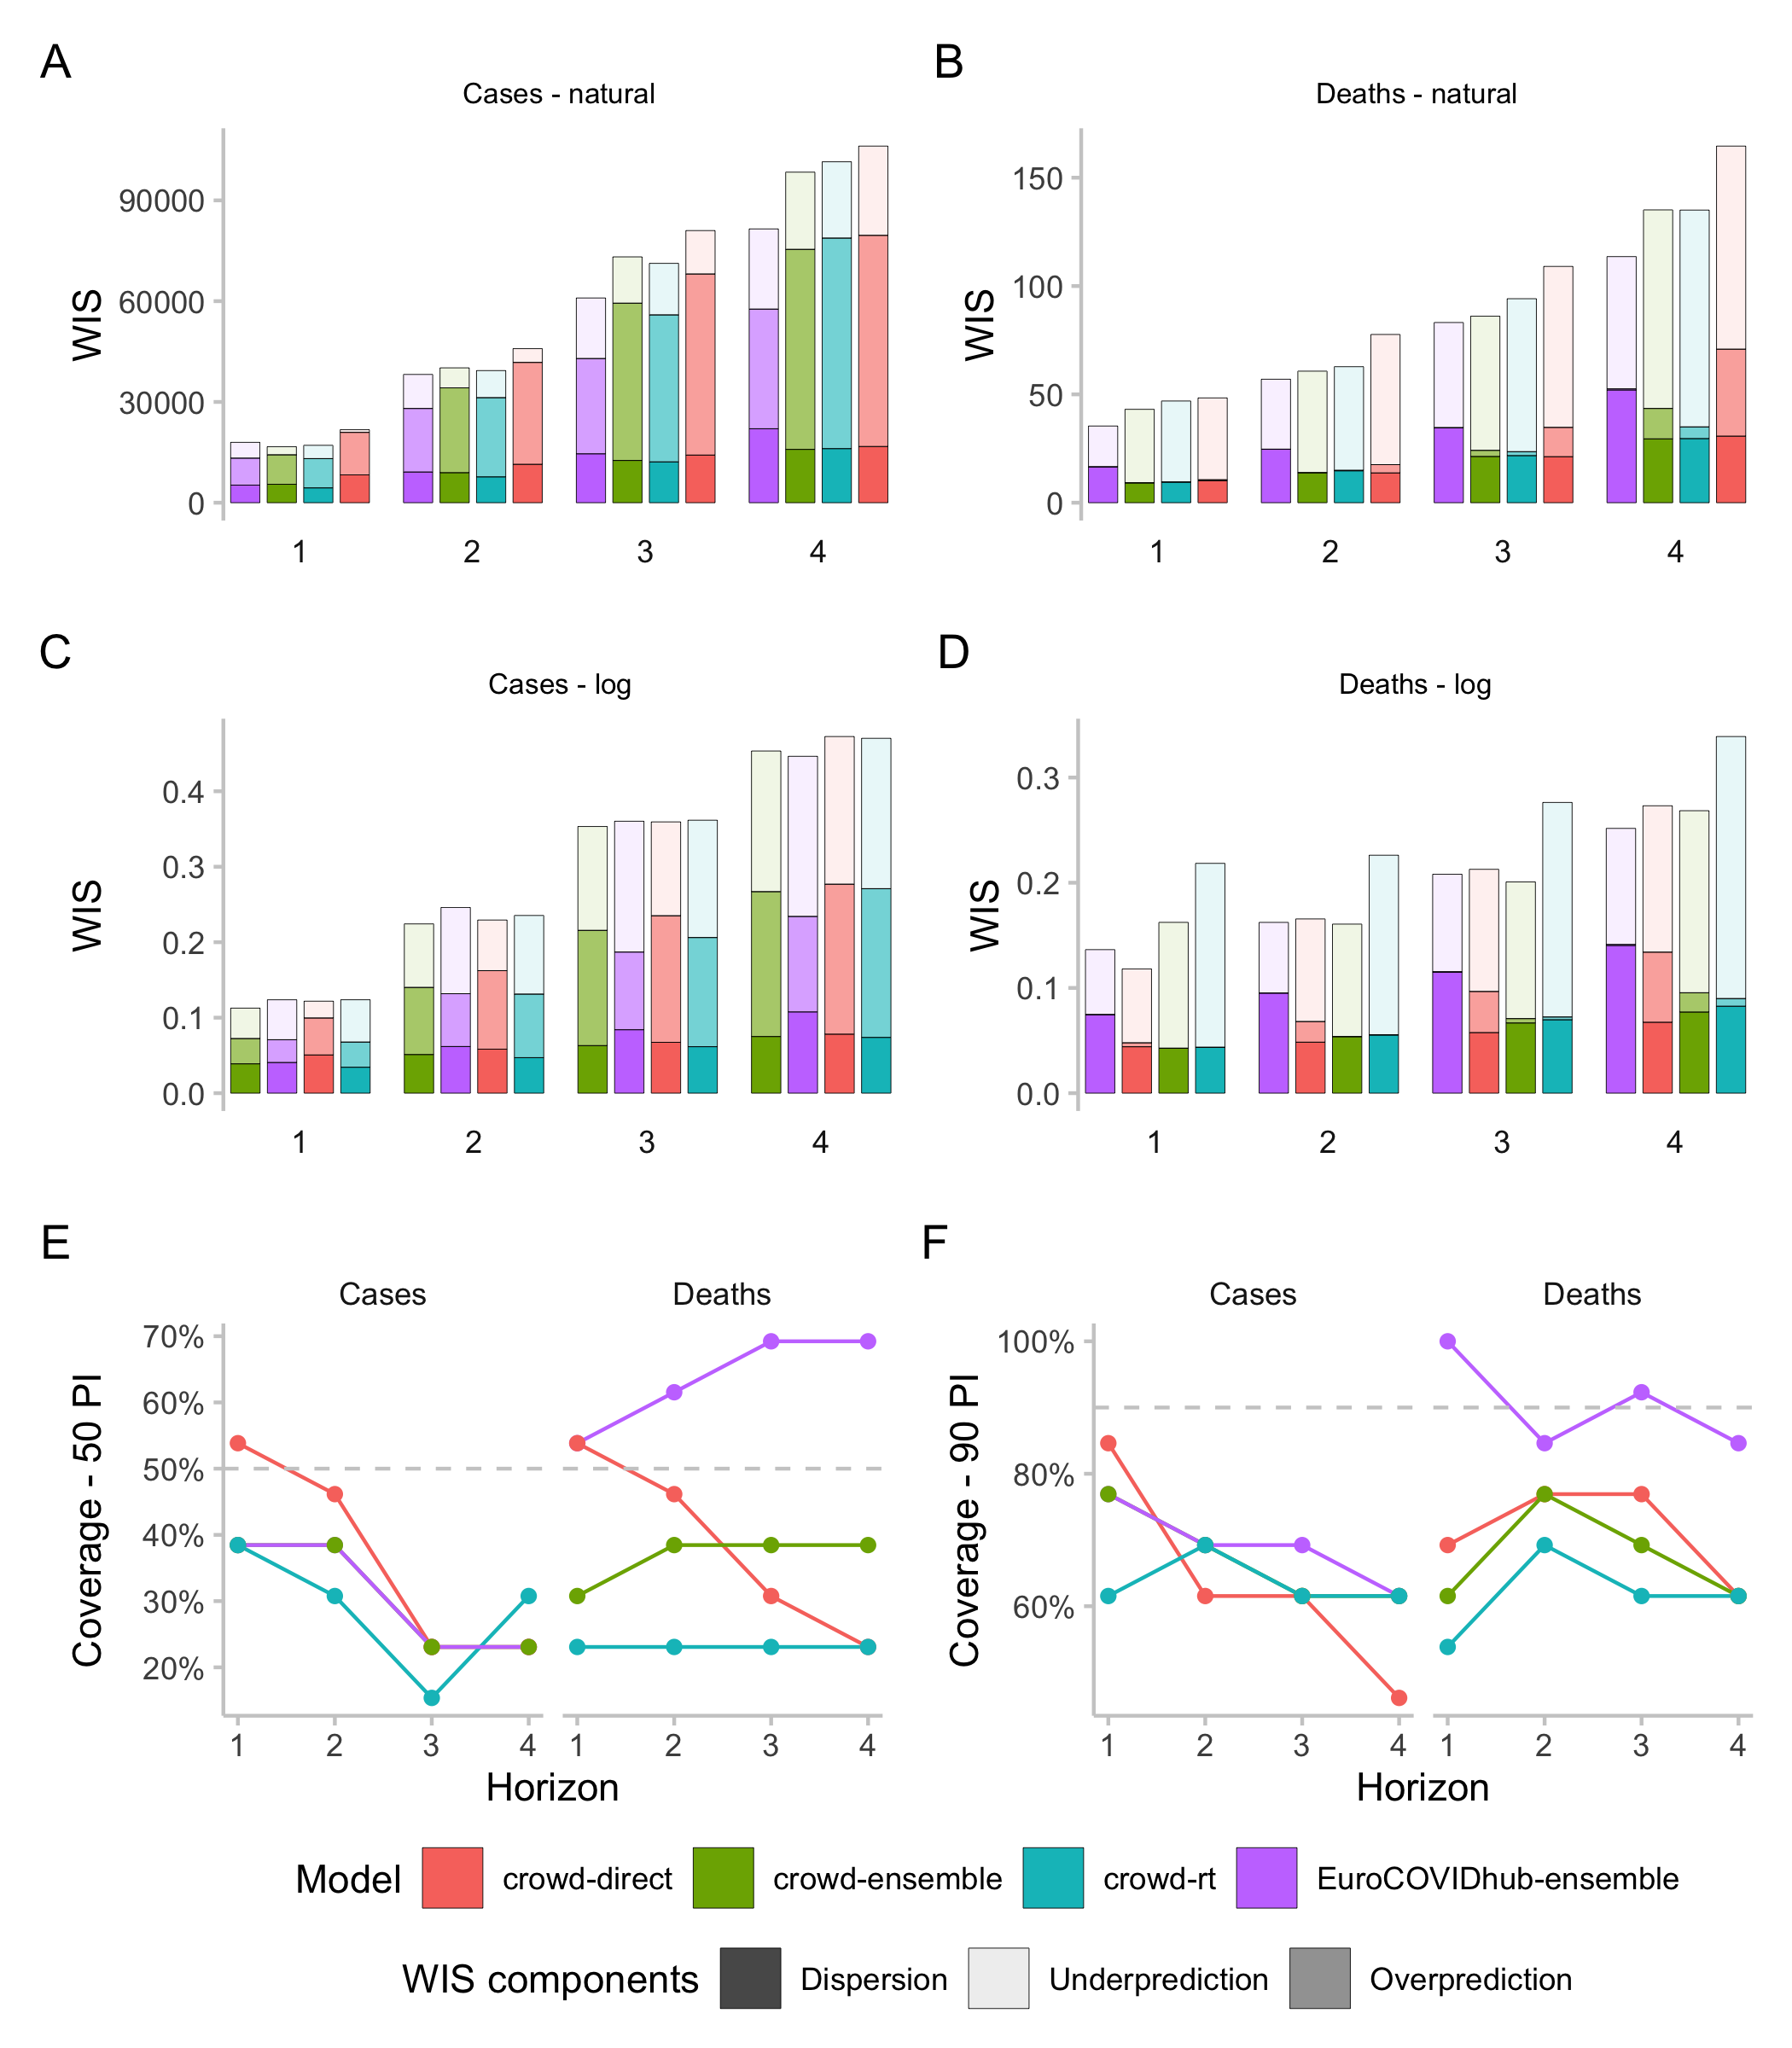
\includegraphics[width=0.99\textwidth]{../output/figures/performance.png}
\caption{\bf{Test}}
\label{fig:performance}
\end{figure}

\subsection*{Case forecasts}

For two-week-ahead-forecasts of incident cases, the Forecast Hub ensemble outperformed all crowd forecasting ensembles as measured by the weighted interval score (WIS). On the natural scale, the WIS as a measure of the absolute distance between forecast and observation increases or decreases with the magnitude of the forecast target \cite{bosseTransformationForecastsEvaluating2023, bracherEvaluatingEpidemicForecasts2021}. Average scores are therefore dominated by performance around the peak when cases were highest, in particular by forecasts made on the 19th of July for the 31st of July \ref{fig:forecasts-scores}. Direct forecasts tended to be higher throughout the study period and especially during the peak than both the $R_t$ forecasts and the Forecast Hub ensemble and therefore showed the poorest performance (see Figure \ref{fig:performance} and Table \ref{tab:scores}). When looking at WIS values on the log scale (that is, when log-transforming forecasts and observations prior to applying the WIS), scores are more equally distributed across the study period and more weight is given to forecasts in June and July which underpredicted the extent to which case number would rise. On the log scale, the Forecast Hub ensemble performs slightly worse than all of the human forecasting approaches. Similarly to what was observed previously \citep{bosseComparingHumanModelbased2022, sherrattPredictivePerformanceMultimodel2022a}, all crowd forecasts as well the Forecast Hub ensemble, exhibited underdispersion, meaning that forecasts on average were too narrow and not uncertain enough, with empirical coverage below nominal coverage.  

\begin{table}[!h]
\centering
\resizebox{\linewidth}{!}{
\begin{tabular}{llcccc}
\toprule
Model & Target & WIS & WIS (log scale) & Coverage 50\% & Coverage 90\%\\
\midrule
EuroCOVIDhub-ensemble & Cases & 38000 & 0.25 & 0.38 & 0.69\\
crowd-direct & Cases & 46000 & 0.23 & 0.46 & 0.62\\
crowd-ensemble & Cases & 40000 & 0.22 & 0.38 & 0.69\\
crowd-rt & Cases & 39000 & 0.24 & 0.31 & 0.69\\
\addlinespace
EuroCOVIDhub-ensemble & Deaths & 57 & 0.16 & 0.62 & 0.85\\
crowd-direct & Deaths & 78 & 0.17 & 0.46 & 0.77\\
crowd-ensemble & Deaths & 61 & 0.16 & 0.38 & 0.77\\
crowd-rt & Deaths & 63 & 0.23 & 0.23 & 0.69\\
\bottomrule
\end{tabular}}
\caption{Table caption}
\label{tab:scores}
\end{table}


\subsection*{Death forecasts} 

In terms of the WIS the Forecast Hub ensemble also outperformed all human forecasts when forecasting deaths. This is true as well for WIS values obtained after applying a log-transformation. From June to the end of July, direct forecasts of deaths were noticeable higher than $R_t$ death forecasts, whereas in August direct death forecasts were substantially lower than $R_t$ death forecasts. On the natural scale, the largest scores occured at the end of the study period when deaths were highest. Direct forecasts, which most strongly underpredicted deaths in August therefore showed the poorest performance overall. On the log scale, however, underprediction in June and July when death incidences were lower, received more weight and direct crowd forecast outperformed $R_t$ forecasts. \textbf{CHECK WITH OTHER GROUND TRUTH DATA?}. Empirical coverage for deaths seems broadly comparable for all human forecasts, whereas the Forecast Hub ensemble displays noticeably better coverage for deaths than for cases (Figure \ref{fig:performance}E, F). 

% \subsection*{Individual forecasts?}


\section*{Discussion}
The discussion should include the implications of the article results in view of prior work in this field.

- hard to draw conclusions, performance changes depending on how you look at the data. 
- headline result not supported? 
- still some evidence that forecasting deaths is easier for computers
- 

- Rt forecasting worked reasonably well. The interface was a bit clunky. Required more expertise. But a potential way to reduce the workload. 

- interesting that combining Rt and direct forecasts for cases improved performance. 


Limitations
- The tournament setting may have distorted results as people were more eager to participate
- ensemble was better


\section*{Conclusions}
Please state what you think are the main conclusions that can be realistically drawn from the findings in the paper, taking care not to make claims that cannot be supported.

Seems that a model of human forecasters is alright. Combining human and model based output is still interesting. 
interface difficult











\subsection*{Author contributions}
In order to give appropriate credit to each author of an article, the individual
contributions of each author to the manuscript should be detailed in this section. We
recommend using author initials and then stating briefly how they contributed.

\subsection*{Competing interests}
The authors declare no competing interests

\subsection*{Grant information}
Please state who funded the work discussed in this article, whether it is your employer,
a grant funder etc. Please do not list funding that you have that is not relevant to this
specific piece of research. For each funder, please state the funder’s name, the grant
number where applicable, and the individual to whom the grant was assigned.

\subsection*{Acknowledgements}
This section should acknowledge anyone who contributed to the research or the
article but who does not qualify as an author based on the criteria provided earlier
(e.g. someone or an organisation that provided writing assistance). Please state how
they contributed; authors should obtain permission to acknowledge from all those
mentioned in the Acknowledgements section.

Acknowledgement to all forecasters








% =================================== Appendix =============================== %


\appendix
\section*{Supplementary information}
% \renewcommand{\thefigure}{SI.\arabic{figure}}
% \setcounter{figure}{0}
% \renewcommand{\thetable}{SI.\arabic{table}} \setcounter{table}{0}


\subsection*{Weighted interval score}
label{sec:wis}
The weighted interval score (smaller values are better) is a proper scoring rule for quantile forecasts. It converges to the continuos ranked probability score (which itself is a generalisation of the absolute error to probabilistic forecasts) for an increasing number of intervals. The score can be decomposed into a dispersion (uncertainty) component and penalties for over- and underprediction. For a single interval, the score is computed as 
  $$IS_\alpha(F,y) = (u-l) + \frac{2}{\alpha} \cdot (l-y) \cdot 1(y \leq l) + \frac{2}{\alpha} \cdot (y-u) \cdot 1(y \geq u), $$ 
  where $1()$ is the indicator function, $y$ is the true value, and $l$ and $u$ are the $\frac{\alpha}{2}$ and $1 - \frac{\alpha}{2}$ quantiles of the predictive distribution $F$, i.e. the lower and upper bound of a single prediction interval. For a set of $K$ prediction intervals and the median $m$, the score is computed as a weighted sum, 
  $$WIS = \frac{1}{K + 0.5} \cdot \left( w_0 \cdot |y - m| + \sum_{k = 1}^{K} w_k \cdot IS_{\alpha}(F, y) \right), $$
  where $w_k$ is a weight for every interval. Usually, $w_k = \frac{\alpha_k}{2}$ and $w_0 = 0.5$. 
  
  
\begin{figure}[H]
\centering
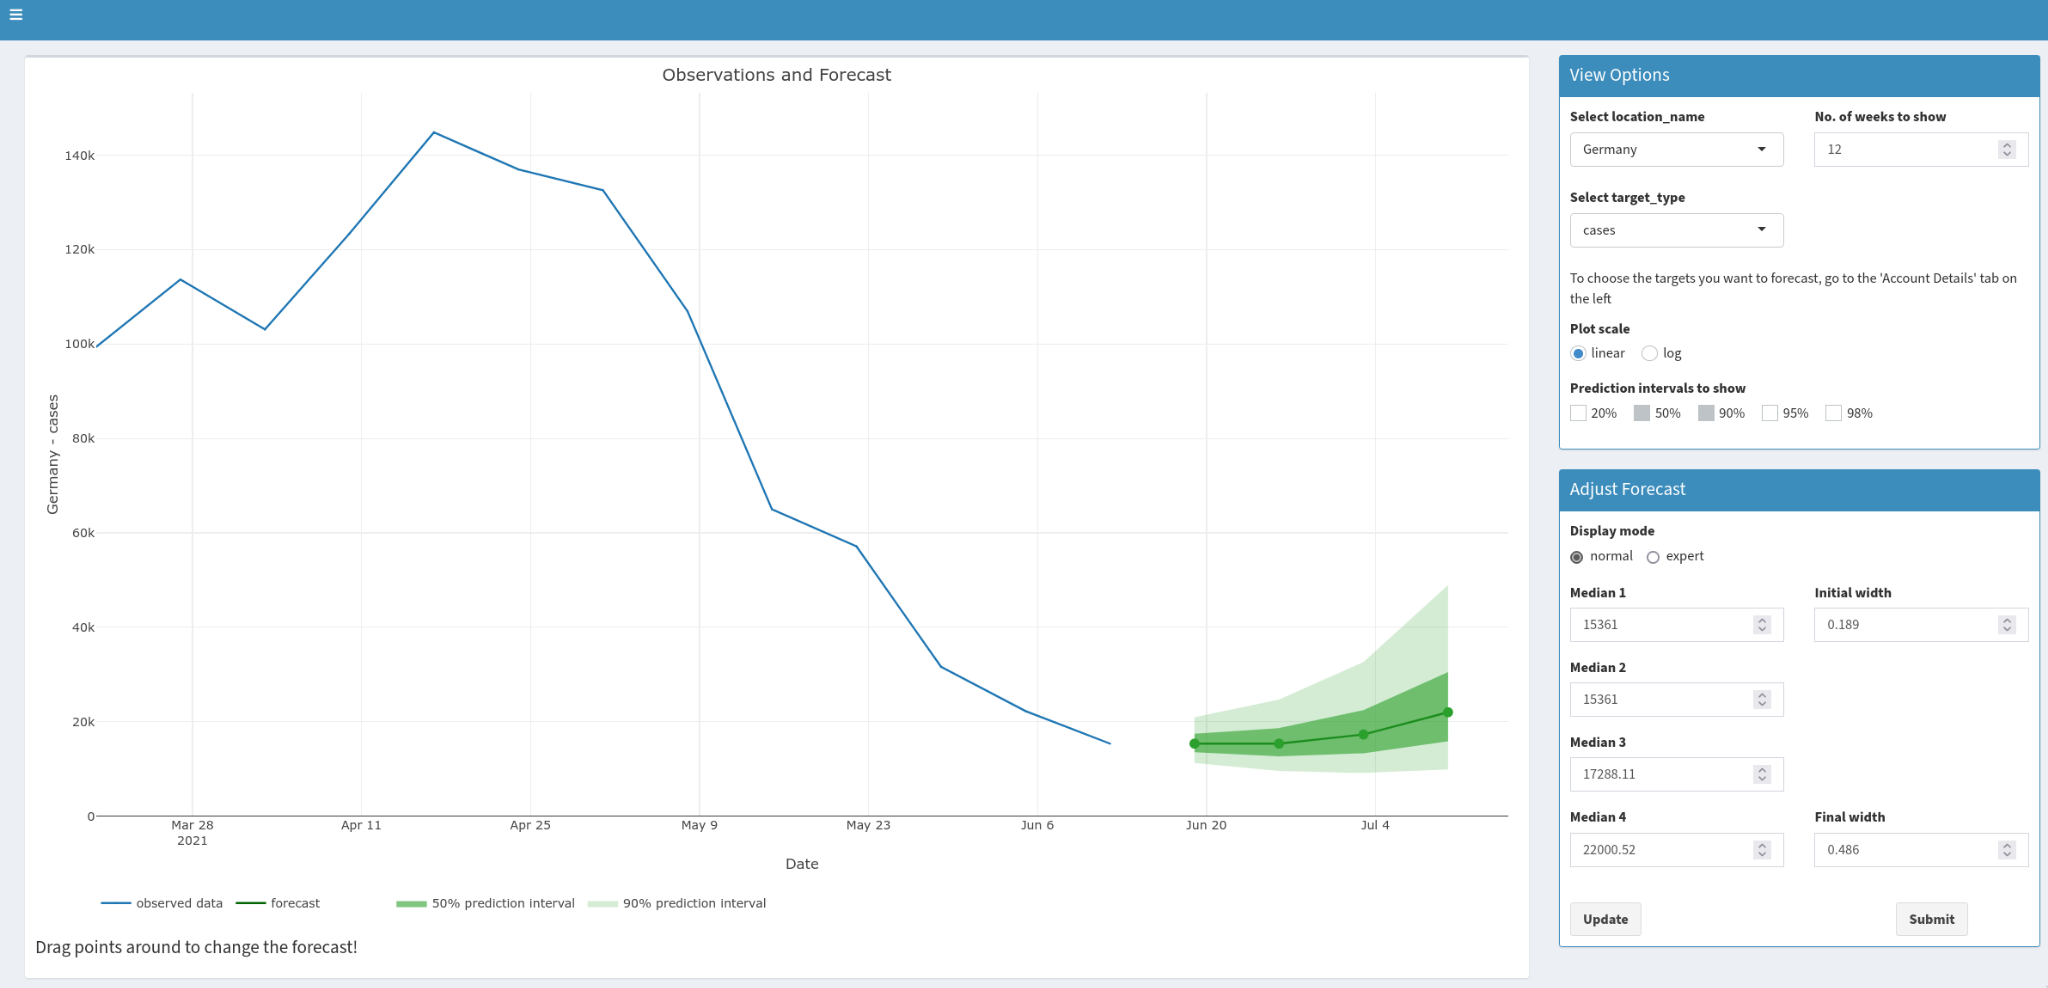
\includegraphics[width=0.99\textwidth]{../output/figures/screenshot-crowd-classical.png}
\caption{\bf{Screenshot of the direct forecasting interface.}}
\label{fig:screenshot-classical}
\end{figure}


\begin{figure}[H]
\centering
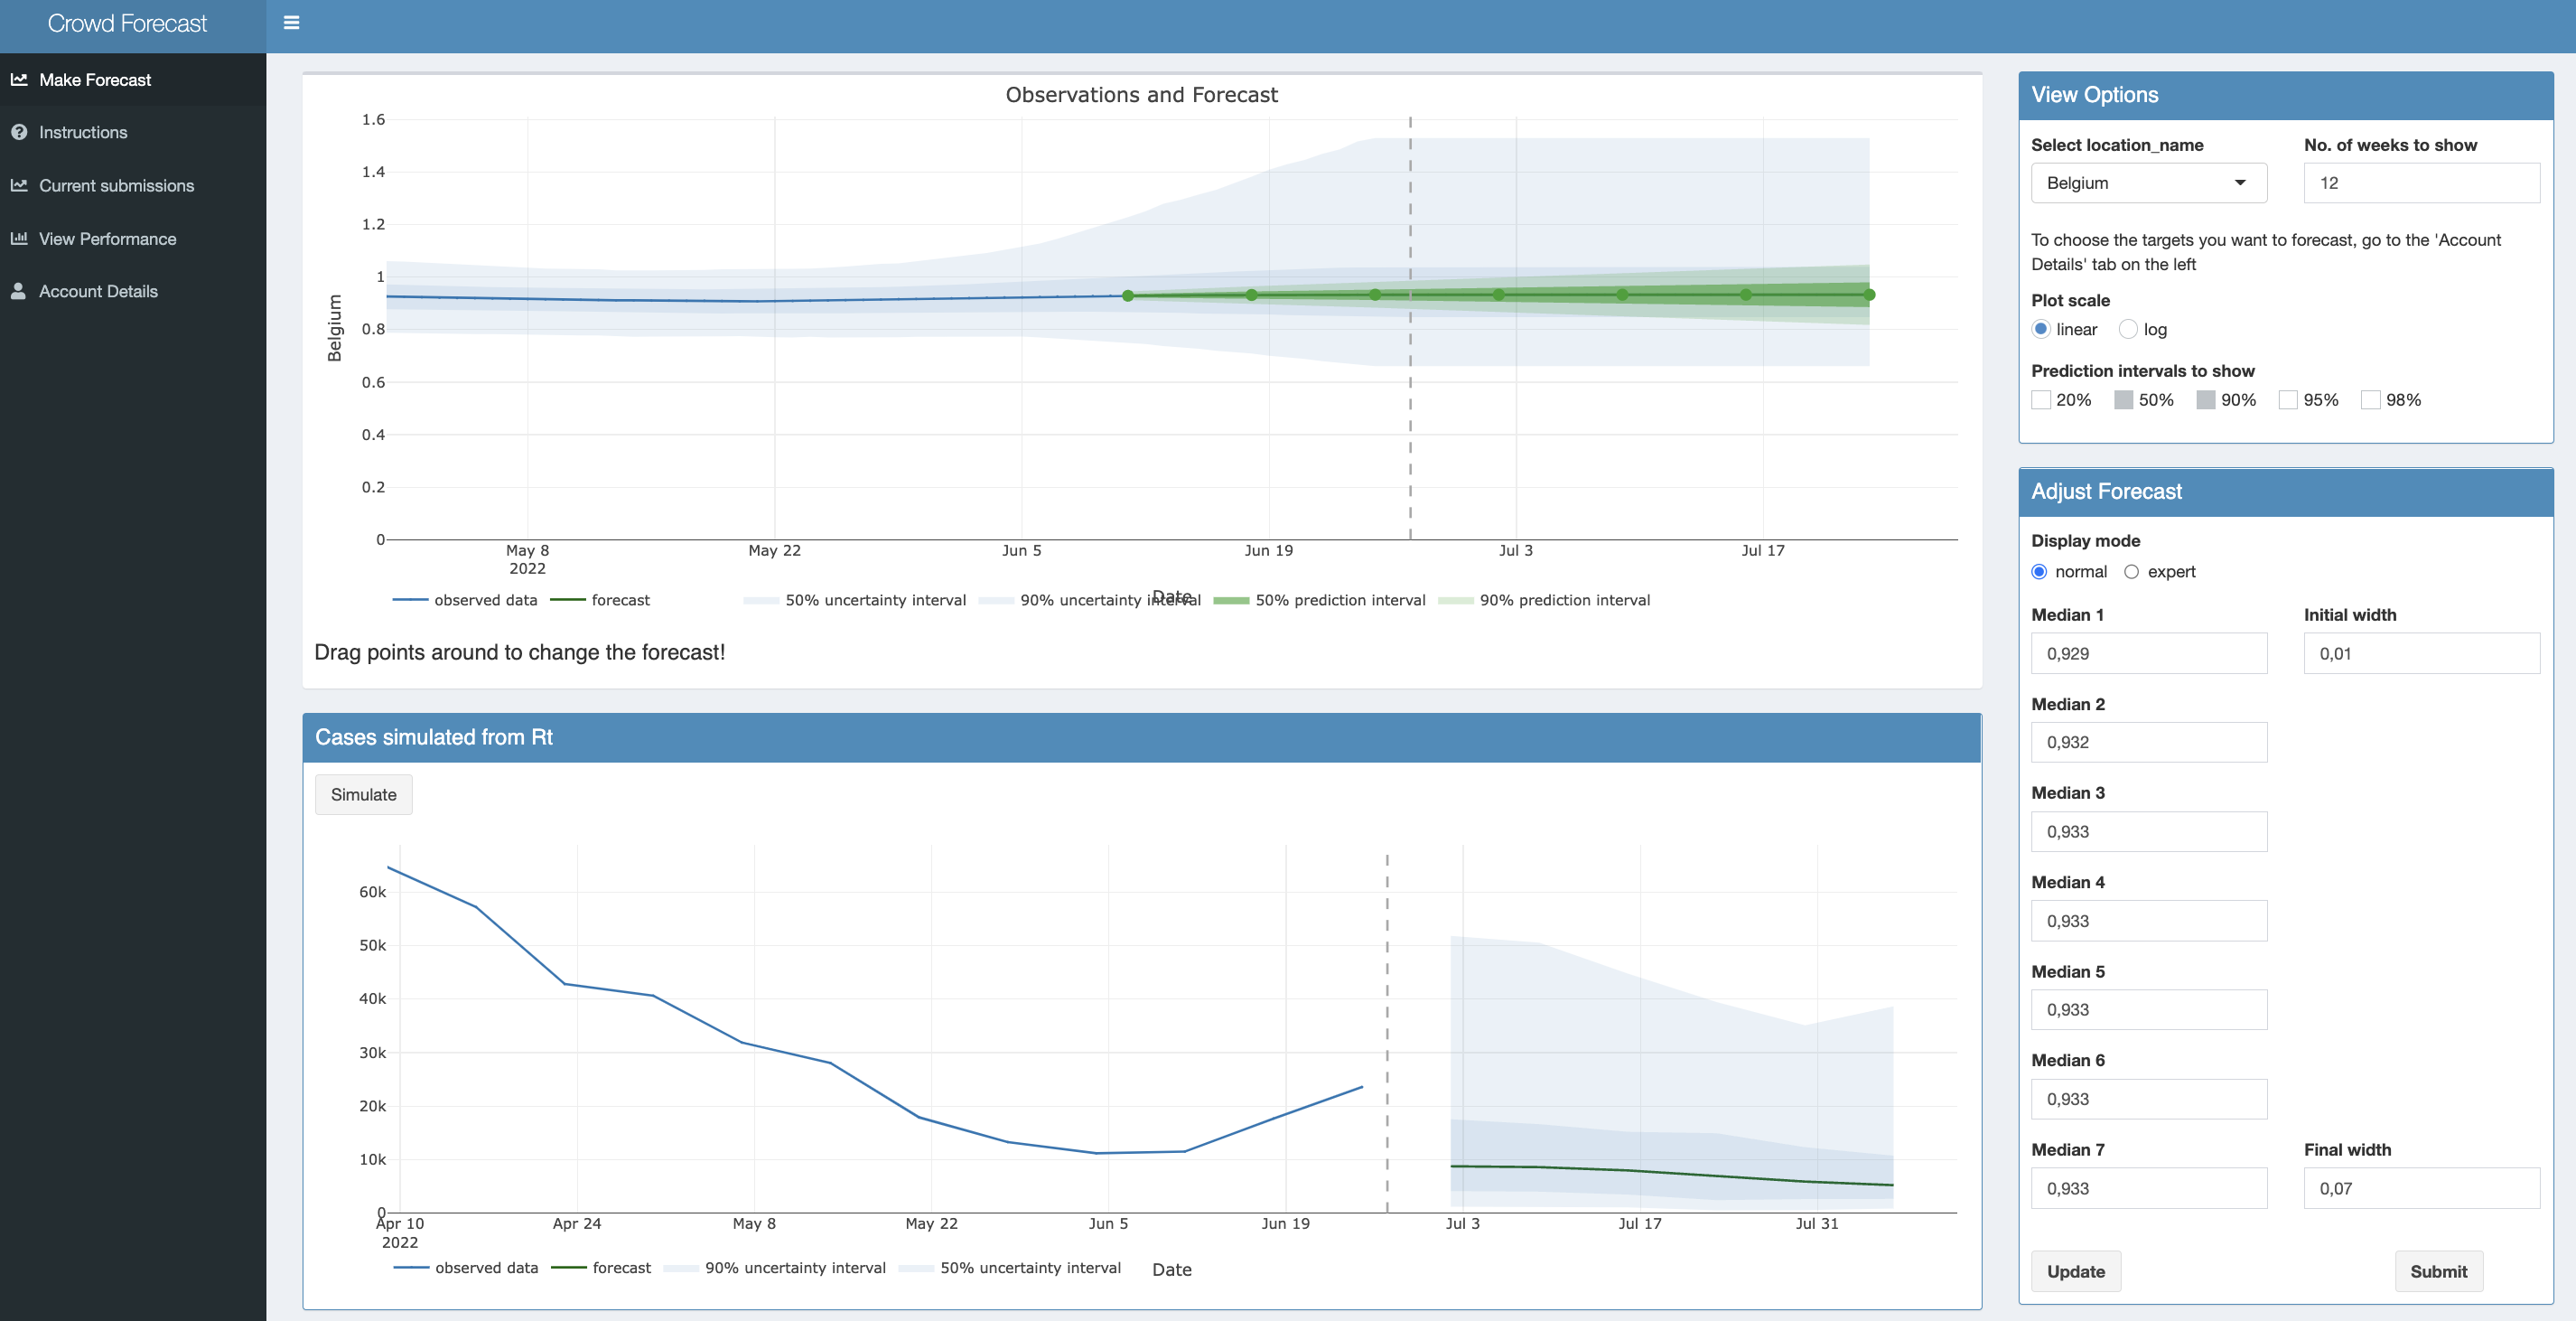
\includegraphics[width=0.99\textwidth]{../output/figures/screenshot-crowd-rt-app.png}
\caption{\bf{Screenshot of the $R_t$ forecasting interface.}}
\label{fig:screenshot-rt}
\end{figure}

\begin{figure}[H]
\centering
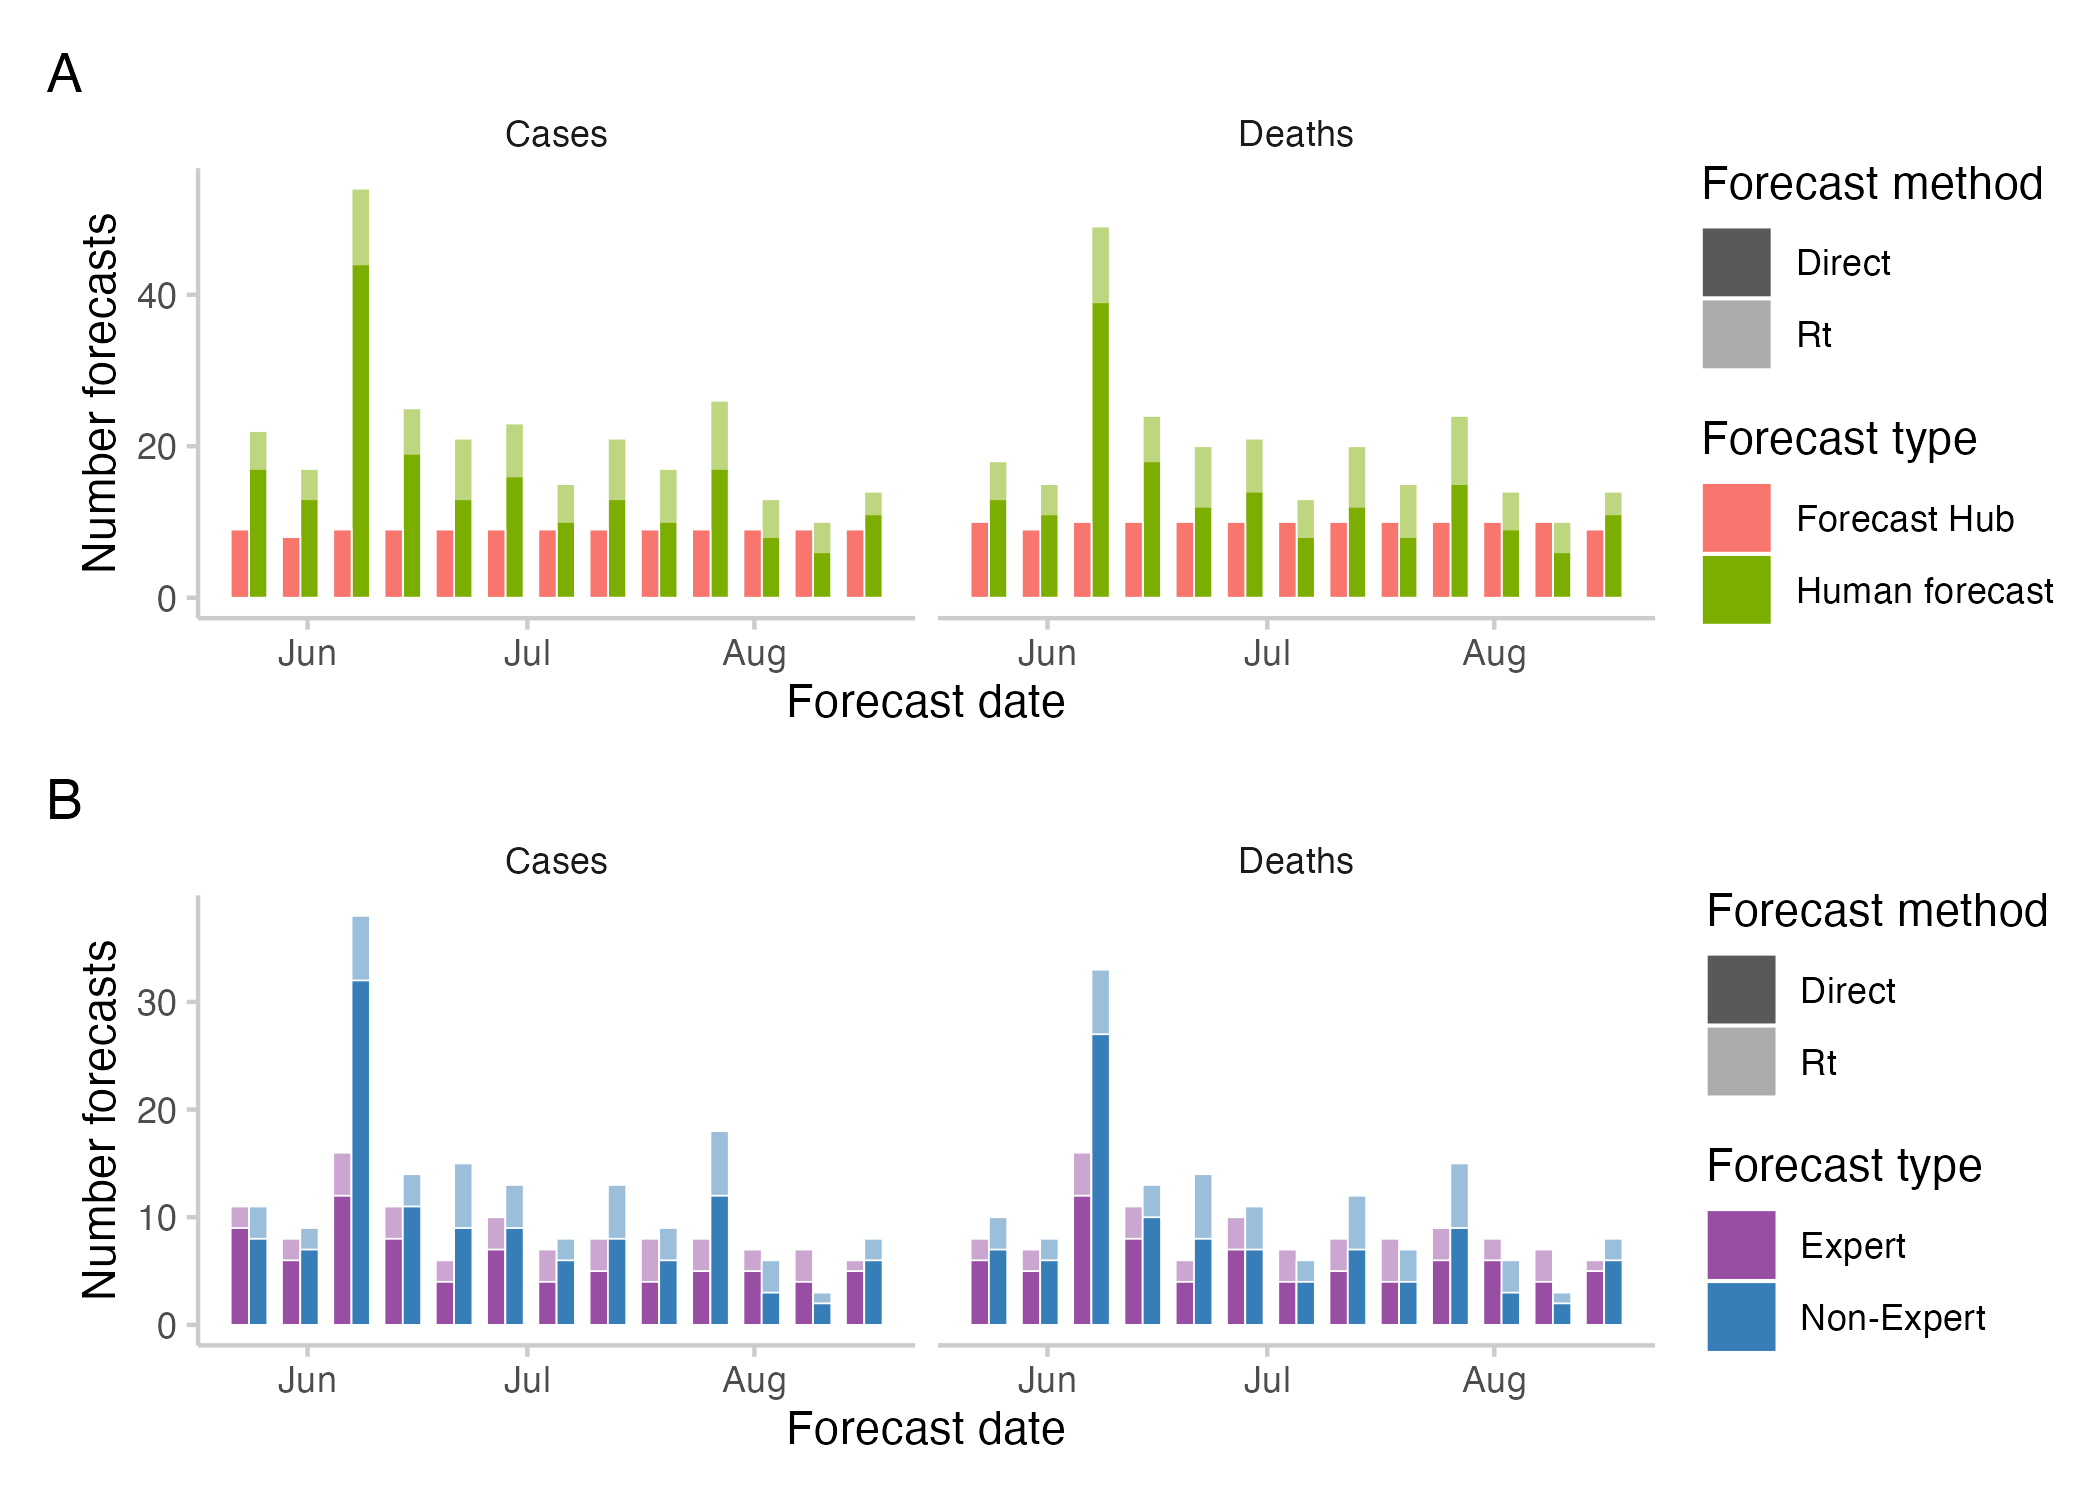
\includegraphics[width=0.99\textwidth]{../output/figures/num-forecasters.png}
\caption{\bf{Number of forecasts across the study period.}}
\label{fig:num-forecasters}
\end{figure}


\clearpage

{\small\bibliographystyle{unsrtnat}
\bibliography{software, uk-forecasting-challenge}}

\bigskip

% See this guide for more information on BibTeX:
% http://libguides.mit.edu/content.php?pid=55482&sid=406343

% For more author guidance please see:
% http://wellcomeopenresearch.org/for-authors/article-guidelines

% When all authors are happy with the paper, use the 
% ‘Submit to WELLCOME OPEN RESEARCH' button from the menu above
% to submit directly to the open life science journal Wellcome Open Research.

% Please note that this template results in a draft pre-submission PDF document.
% Articles will be professionally typeset when accepted for publication.

% We hope you find the Wellcome Open Research Overleaf template useful,
% please let us know if you have any feedback using the help menu above.



\end{document}